% !TEX encoding = UTF-8 Unicode
\documentclass[hyperref={bookmarks=false}]{beamer}
\usetheme{CambridgeUS}
\setbeamercolor{bibliography entry author}{fg=black}
\setbeamercolor{item}{fg=darkred}
\setbeamercolor{caption name}{fg=darkred}
\beamertemplatenavigationsymbolsempty

\usepackage[serbianc]{babel}
\usepackage{type1ec}
\usepackage{cmap}

\graphicspath{{../slike}}

\title[Интерактомика]{Биолошке мреже са фокусом на интерактомику}
\titlegraphic{
\includegraphics[height=3cm,width=3.5cm]{MATF.png}}
\author{Лазар Васовић}
\institute[]{Математички факултет, Универзитет у Београду\\\url{https://github.com/matfija/Neuredjenost-u-interaktomu}}
\date[Математички факултет]{мај 2022}

\begin{document}

\frame{\titlepage}

\begin{frame}{Садржај}
\tableofcontents[subsectionstyle=hide]
\end{frame}

\section{Биолошке мреже}
\subsection{Биолошке мреже}
\begin{frame}{Биолошке мреже}
\begin{itemize}
	\item Биолошки системи, било да је реч о маленој ћелији или огромном екосистему, састоје се од основних градивних јединица, нпр. гена, протеина, метаболита или јединки, које међудејствују.

	\item Ретке су јединице које делују у потпуности самостално, тако да су интеракције кључни део сваког биолошког система. Заправо се ниједан систем не може посматрати као прост збир елемената.

	\item За потребе биоинформатичке анализе, неопходно је одабрати одговарајући математички модел. Природни модел интерагујућих блокова, тиме и биолошких система, јесте граф (мрежа), уз напомену да он ипак не успева да представи све односе.
\end{itemize}
\end{frame}

\subsection{Моделовање биолошког система графом}
\begin{frame}{Моделовање биолошког система графом}
\centering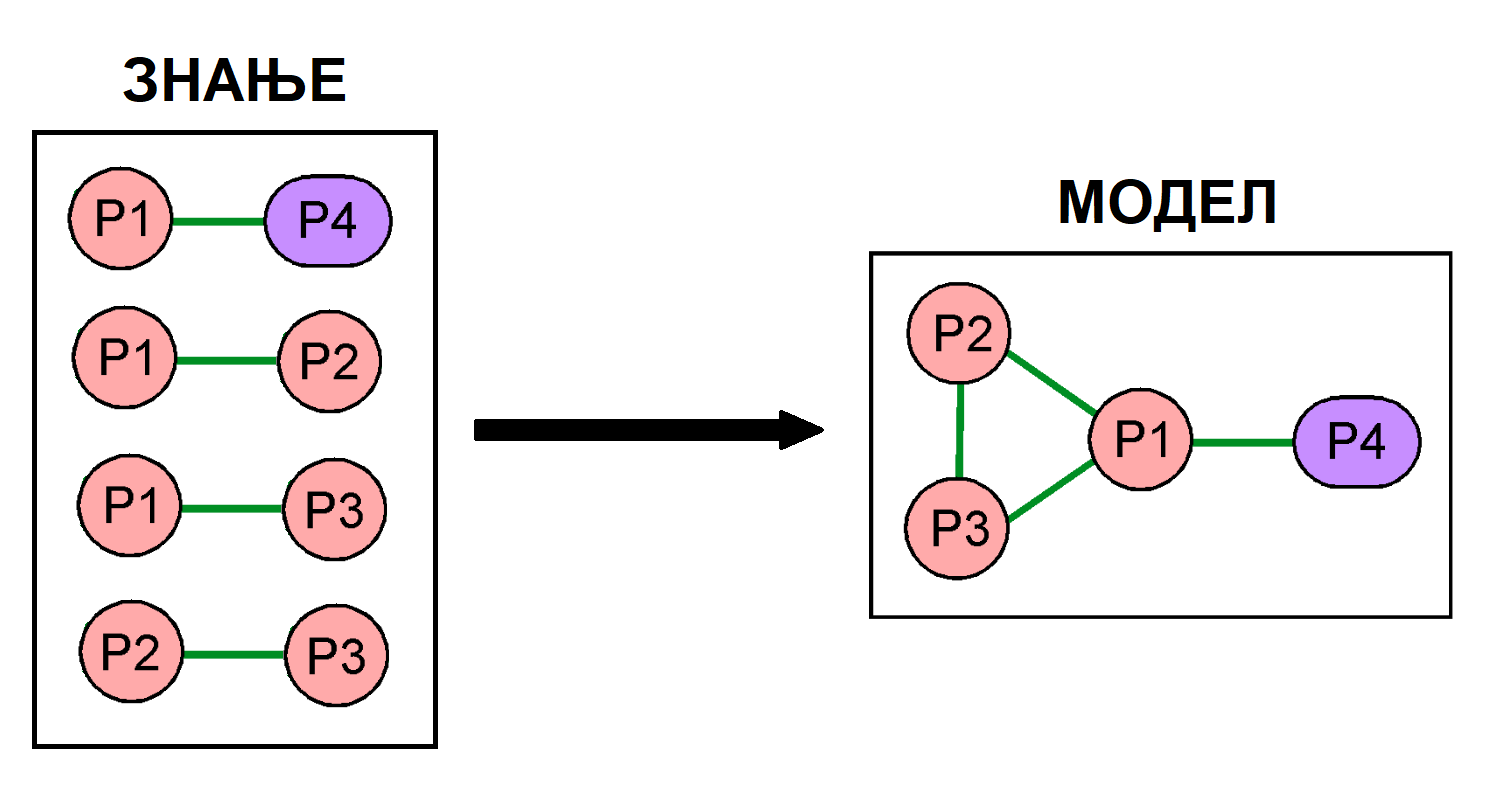
\includegraphics[width=.95\textwidth]{modelovanje.png}
\end{frame}

\subsection{Теорија графова}
\begin{frame}{Теорија графова}
\begin{itemize}
	\item Граф $G$ је уређени пар коначних скупова чворова $V$ (\textit{vertices}) и грана (ивица, веза) $E$ (\textit{edges}). Математички записано, граф $G$ је $G = (V, E)$, скуп $V$ од $n$ чворова $V = \{v_1, ..., v_n\}$, а скуп $E$ од $m$ грана $E = \{e_1, ..., e_m\}$. Грана $e_k = (v_i, v_j)$ повезује чвор $v_i$ са $v_j$.

	\item Уколико није важан смер везе, гране су неуређени парови чворова, а граф је неусмерен. Пример везе: протеинска интеракција.

	\item Уколико јесте важан смер везе, гране су уређени парови чворова, а граф је усмерен (диграф). Пример везе: генски утицај.

	\item Остали важни појмови: пут, циклус, компоненте повезаности, дрво (стабло), мултиграф, графовски алгоритми (нпр. обилазак)...
\end{itemize}
\end{frame}

\subsection{Једноставан пример графа}
\begin{frame}{Једноставан пример графа}
\centering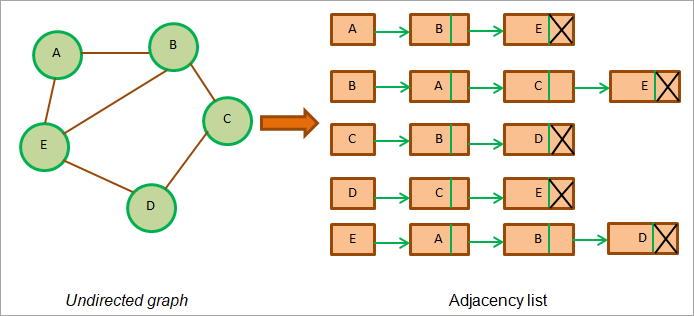
\includegraphics[width=.95\textwidth]{graf.png}
\end{frame}

\subsection{Особине биолошких мрежа}
\begin{frame}{Особине биолошких мрежа}
\begin{itemize}
	\item Мере централности претпостављају значај чвора у мрежи.
	\begin{itemize}
		\item Степен чвора (централност степена) -- број суседа у мрежи.
	\end{itemize}

	\item Тополошке карактеристике графа описују целокупну мрежу.
	\begin{itemize}
		\item Пречник (\textit{diameter}, $D$) -- максимална дужина најкраћег пута.
		\item Карактеристична дужина пута (\textit{average path length}, $L$) -- просечна дужина најкраћих путева између свака два чвора.
		\item Коефицијент груписања (\textit{clustering coefficient}, $CC$) -- просечна склоност чворова да граде густо повезане групе (кластере).
		\item Расподела степена (\textit{degree distribution}, $P_k$) -- вероватноћа $k$.
	\end{itemize}

	\item Очекују се мање вредности $D$ и $L$ („мали свет”), као и велики $CC$ (јака структура заједнице). Расподела чворова је углавном степена (\textit{power law} или \textit{scale-free}, $P_k \sim k^{-\gamma}$), према којој већина чворова има мали број суседа, уз мањи број високоповезаних хабова.
\end{itemize}
\end{frame}

\subsection{Сложенији примери графова}
\begin{frame}{Сложенији примери графова}
\centering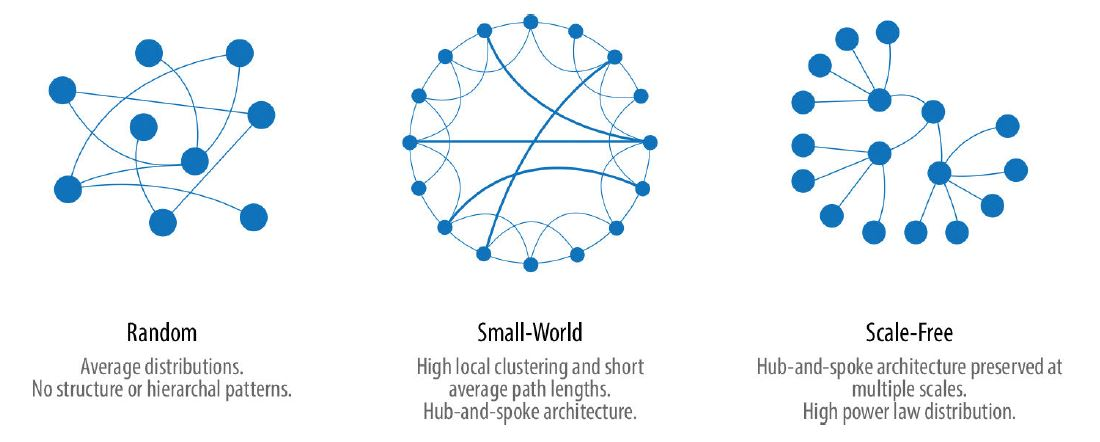
\includegraphics[width=.95\textwidth]{osobine.jpg}
\end{frame}

\subsection{Сложеније поређење графова}
\begin{frame}{Сложеније поређење графова}
\centering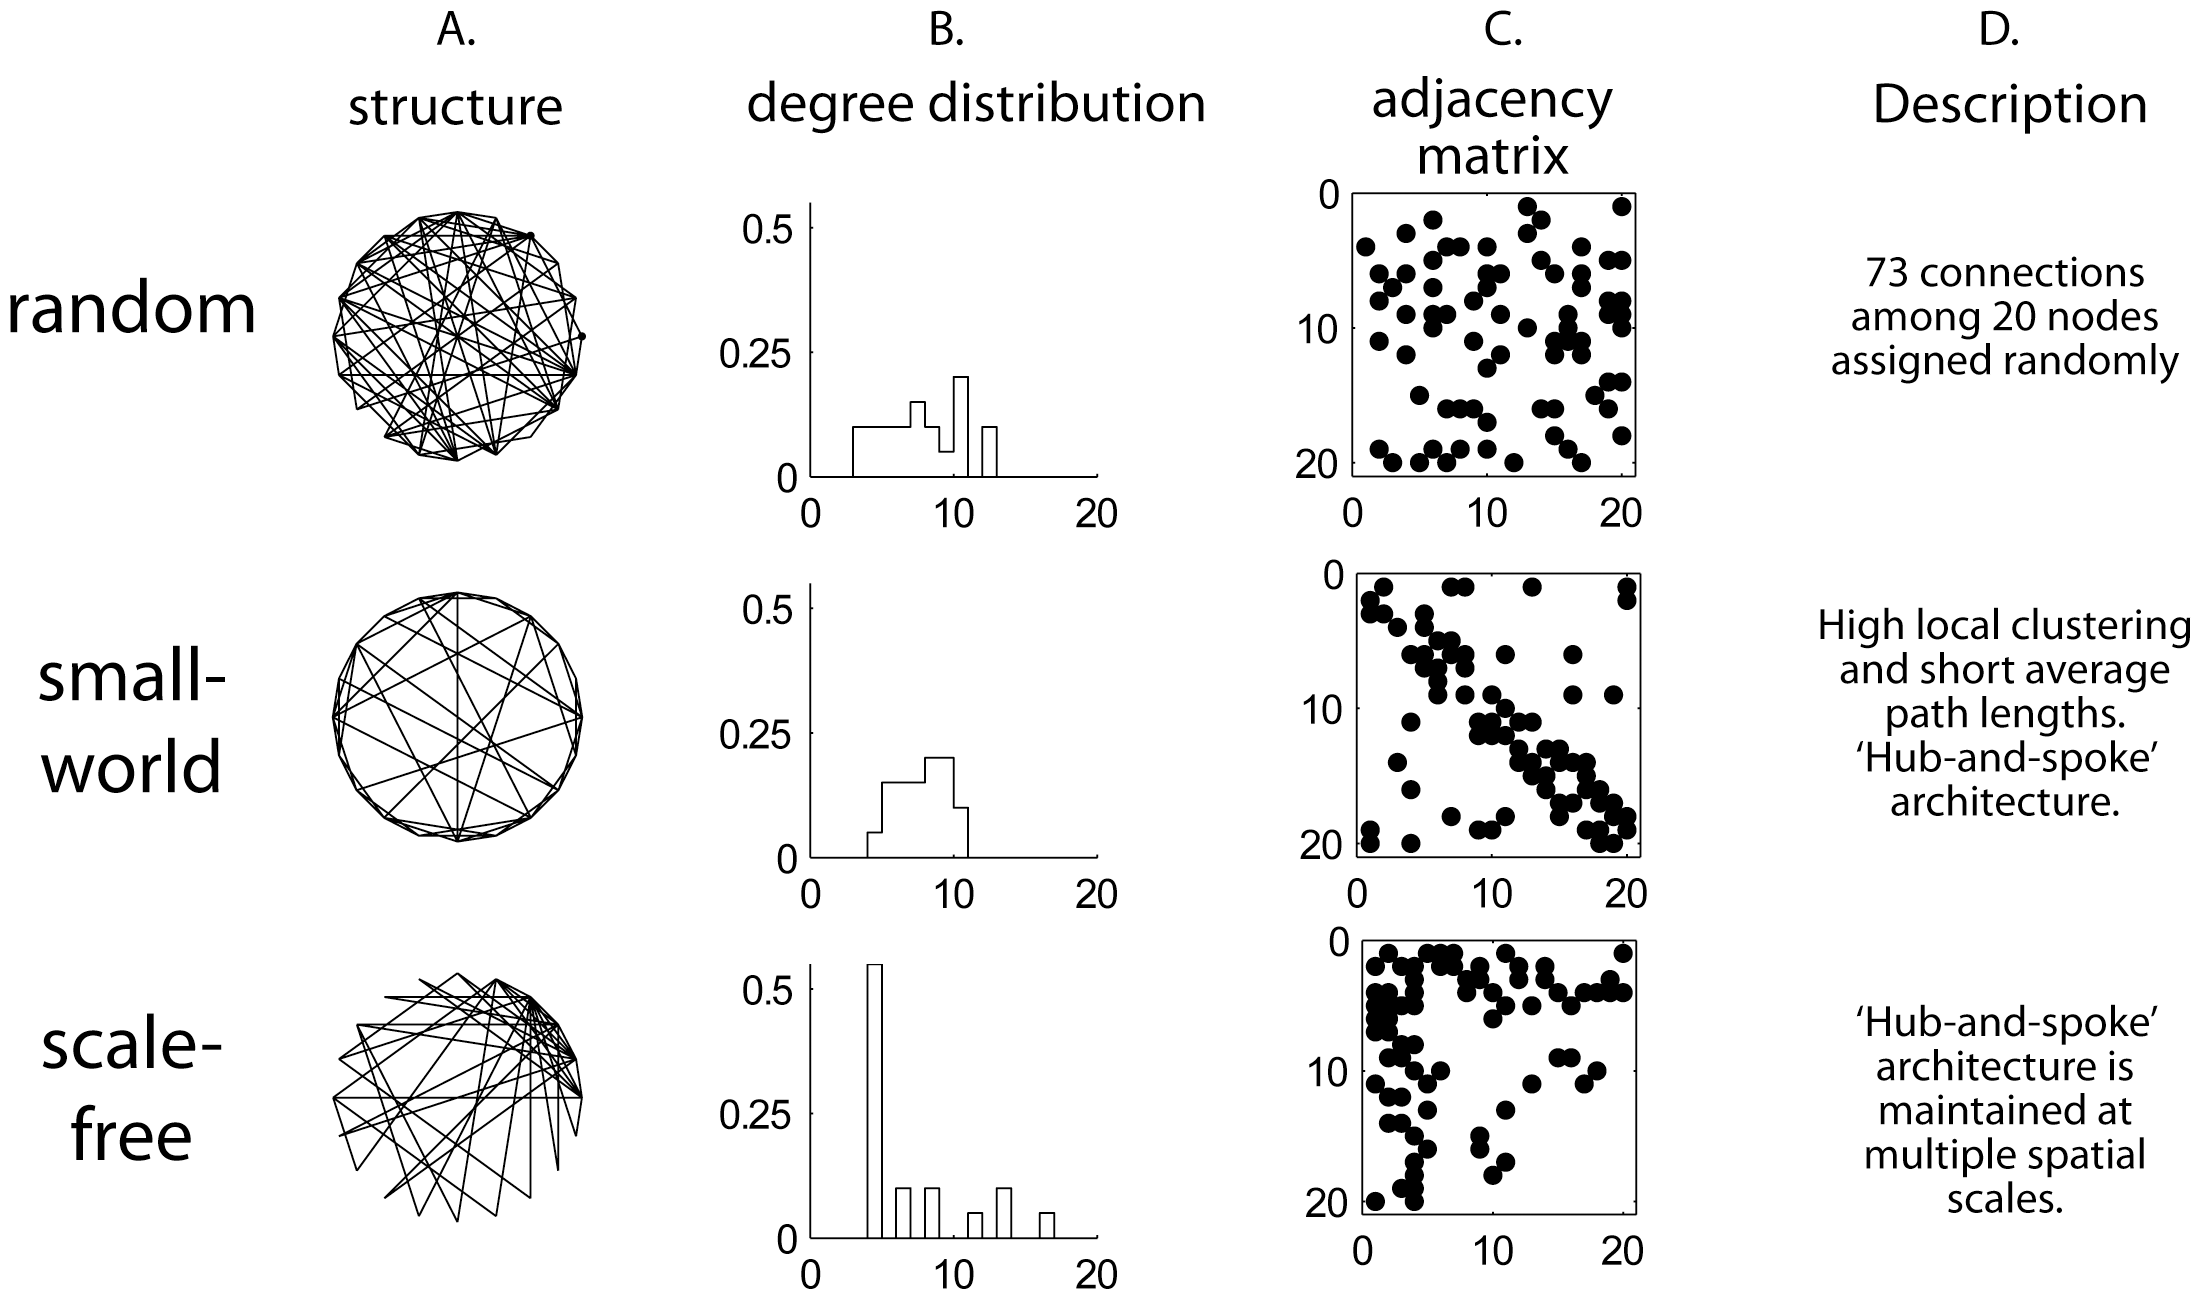
\includegraphics[width=.95\textwidth]{osobine2.png}
\end{frame}

\subsection{Врсте биолошких мрежа}
\begin{frame}{Врсте биолошких мрежа}
\begin{itemize}
	\item Биолошке мреже могу се поделити према величини и врсти основних градивних јединица моделованог биолошког система, представљених чвором графа, као и природи интеракције.

	\item Мале (микроскопске) мреже:
	\begin{itemize}
		\item регулаторне мреже гена (\textit{gene regulatory network}, $GRN$),
		\item мреже преноса сигнала (\textit{signal transduction network}, $STN$),
		\item мреже протеинских интеракција (\textit{protein interaction network}, $PIN$),
		\item метаболичке мреже (\textit{metabolic network}).
	\end{itemize}

	\item Велике (макроскопске) мреже:
	\begin{itemize}
		\item филогенетске мреже (\textit{phylogenetic network}),
		\item еколошке мреже (\textit{ecological network}).
	\end{itemize}

	\item Постоје и разне друге врсте мрежа, нпр. мождана (конектом).
\end{itemize}
\end{frame}

\subsection{Пример генске регулације}
\begin{frame}{Пример генске регулације}
\centering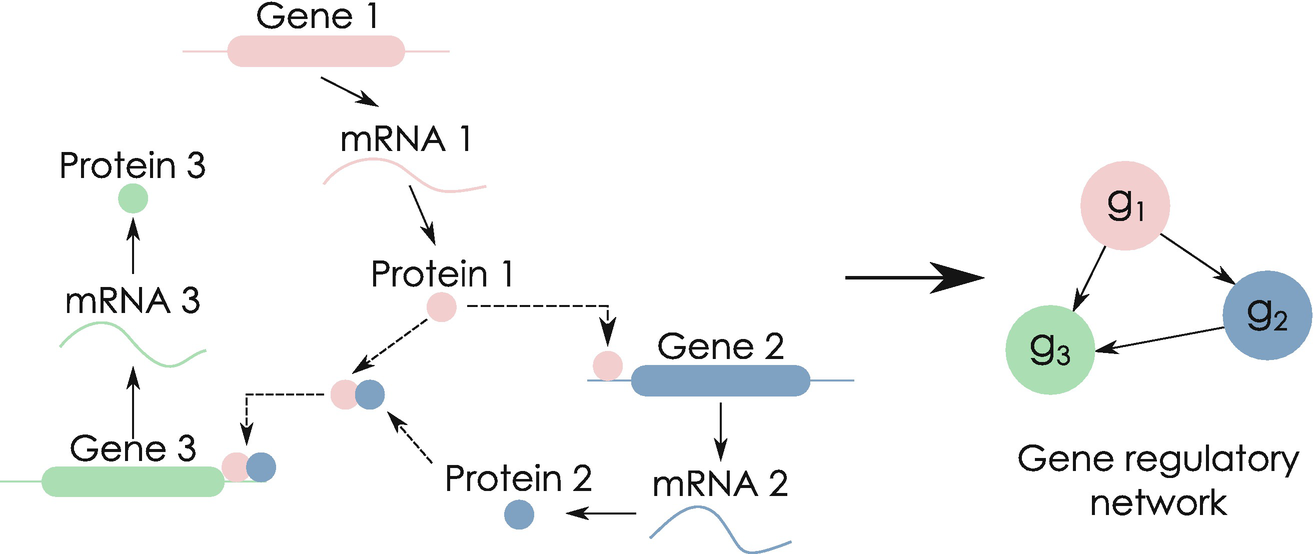
\includegraphics[width=.95\textwidth]{GRN.jpg}
\end{frame}

\subsection{Сигнални путеви људске ћелије}
\begin{frame}{Сигнални путеви људске ћелије}
\centering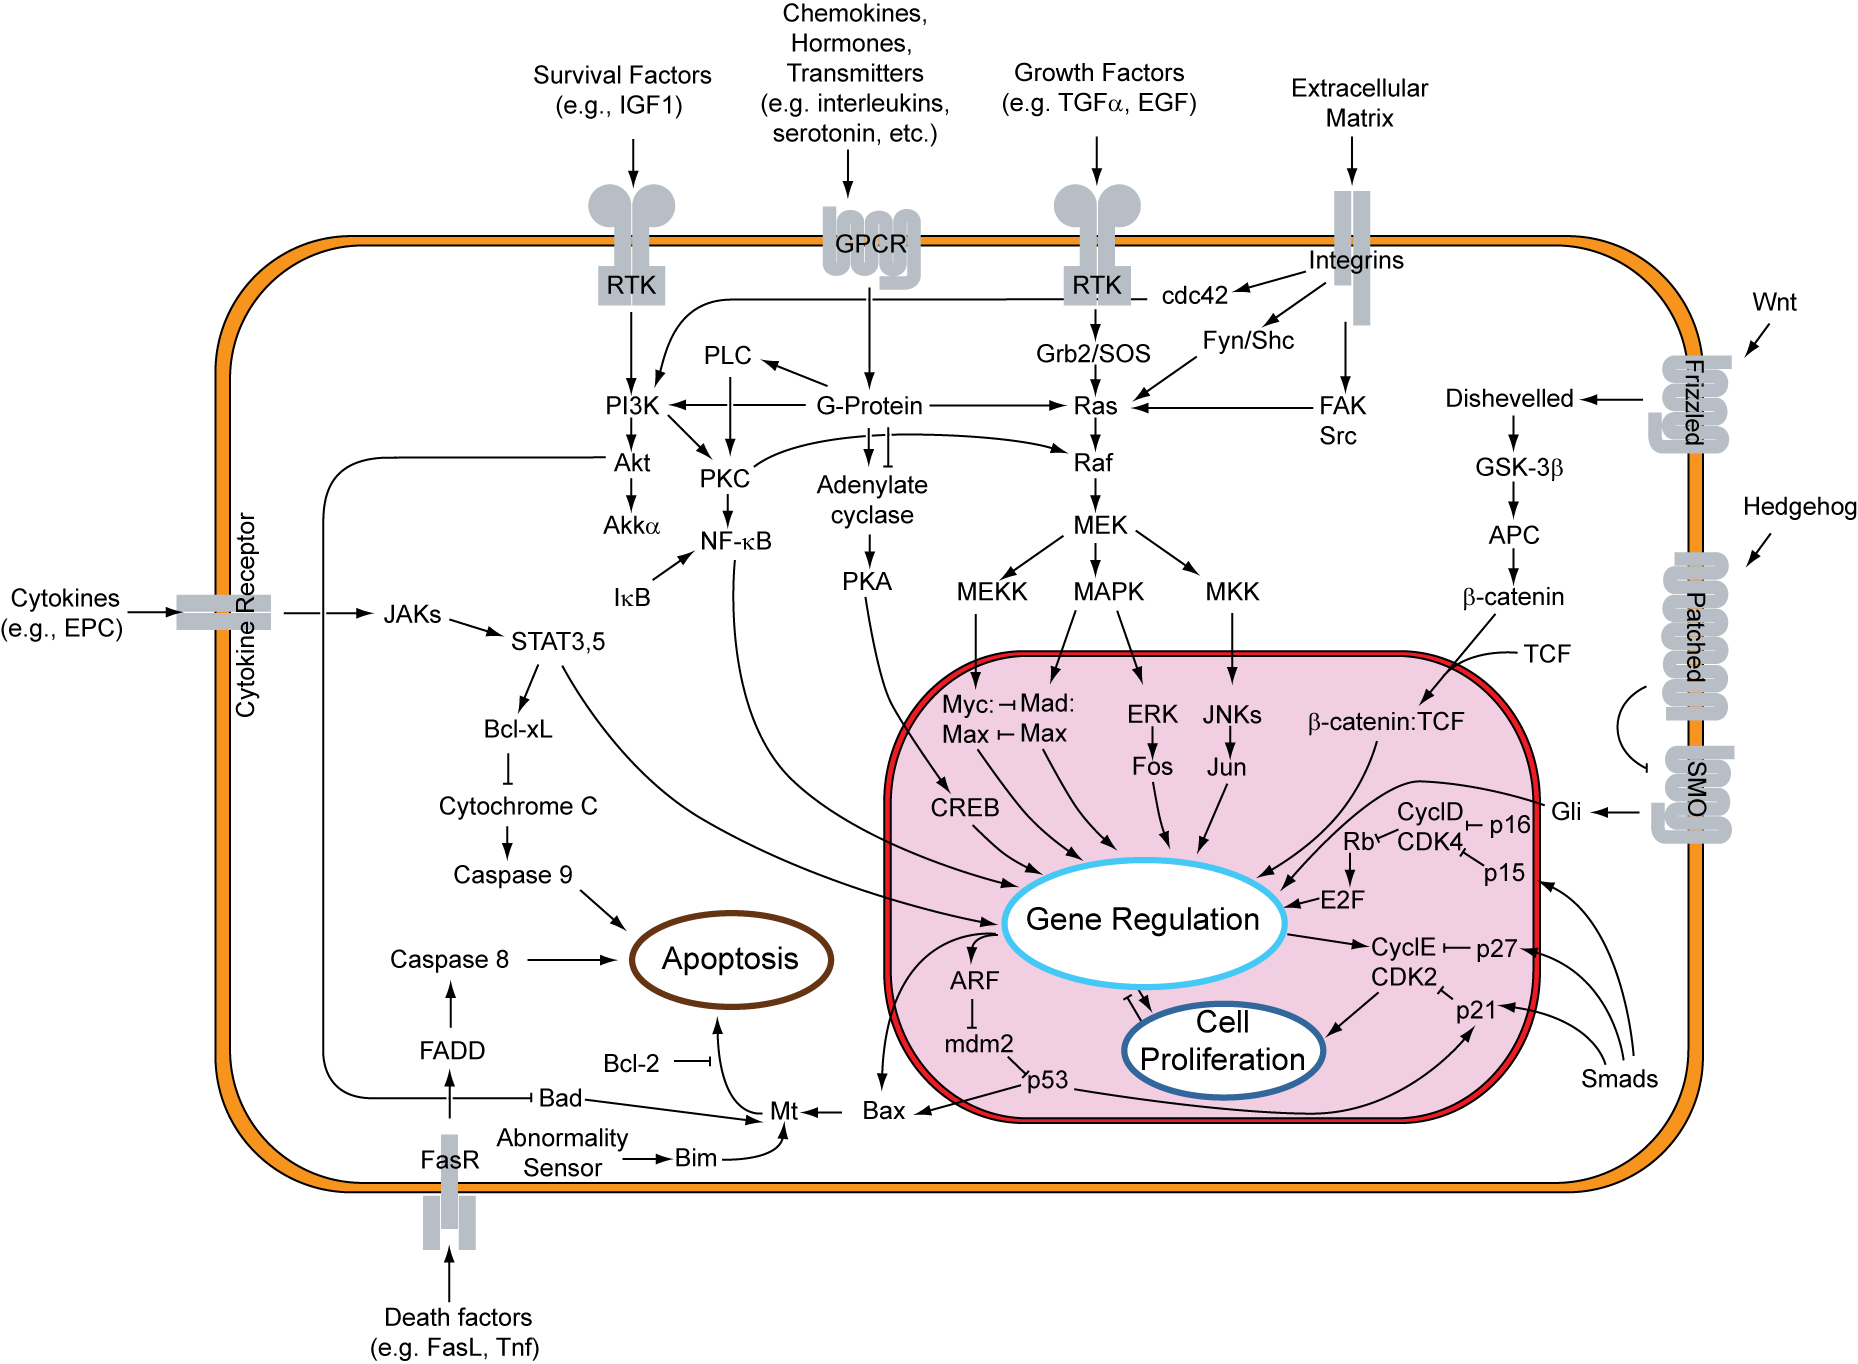
\includegraphics[width=.85\textwidth]{STN.png}
\end{frame}

\subsection{Кребсов циклус}
\begin{frame}{Кребсов циклус}
\centering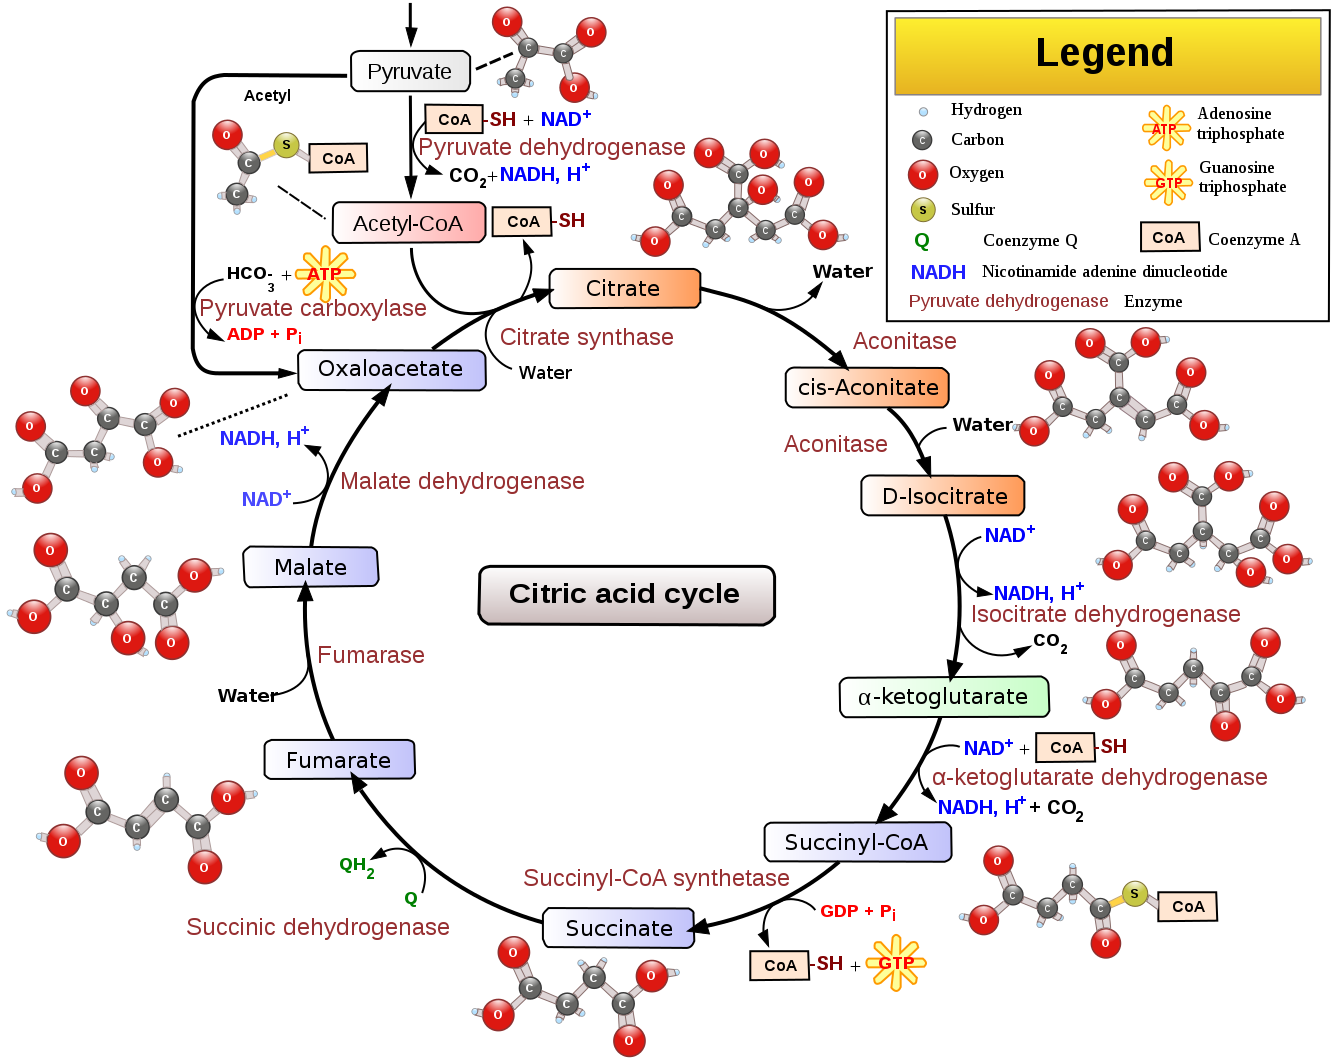
\includegraphics[width=.8\textwidth]{Krebs.png}
\end{frame}

\subsection{Дрво живота}
\begin{frame}{Дрво живота}
\centering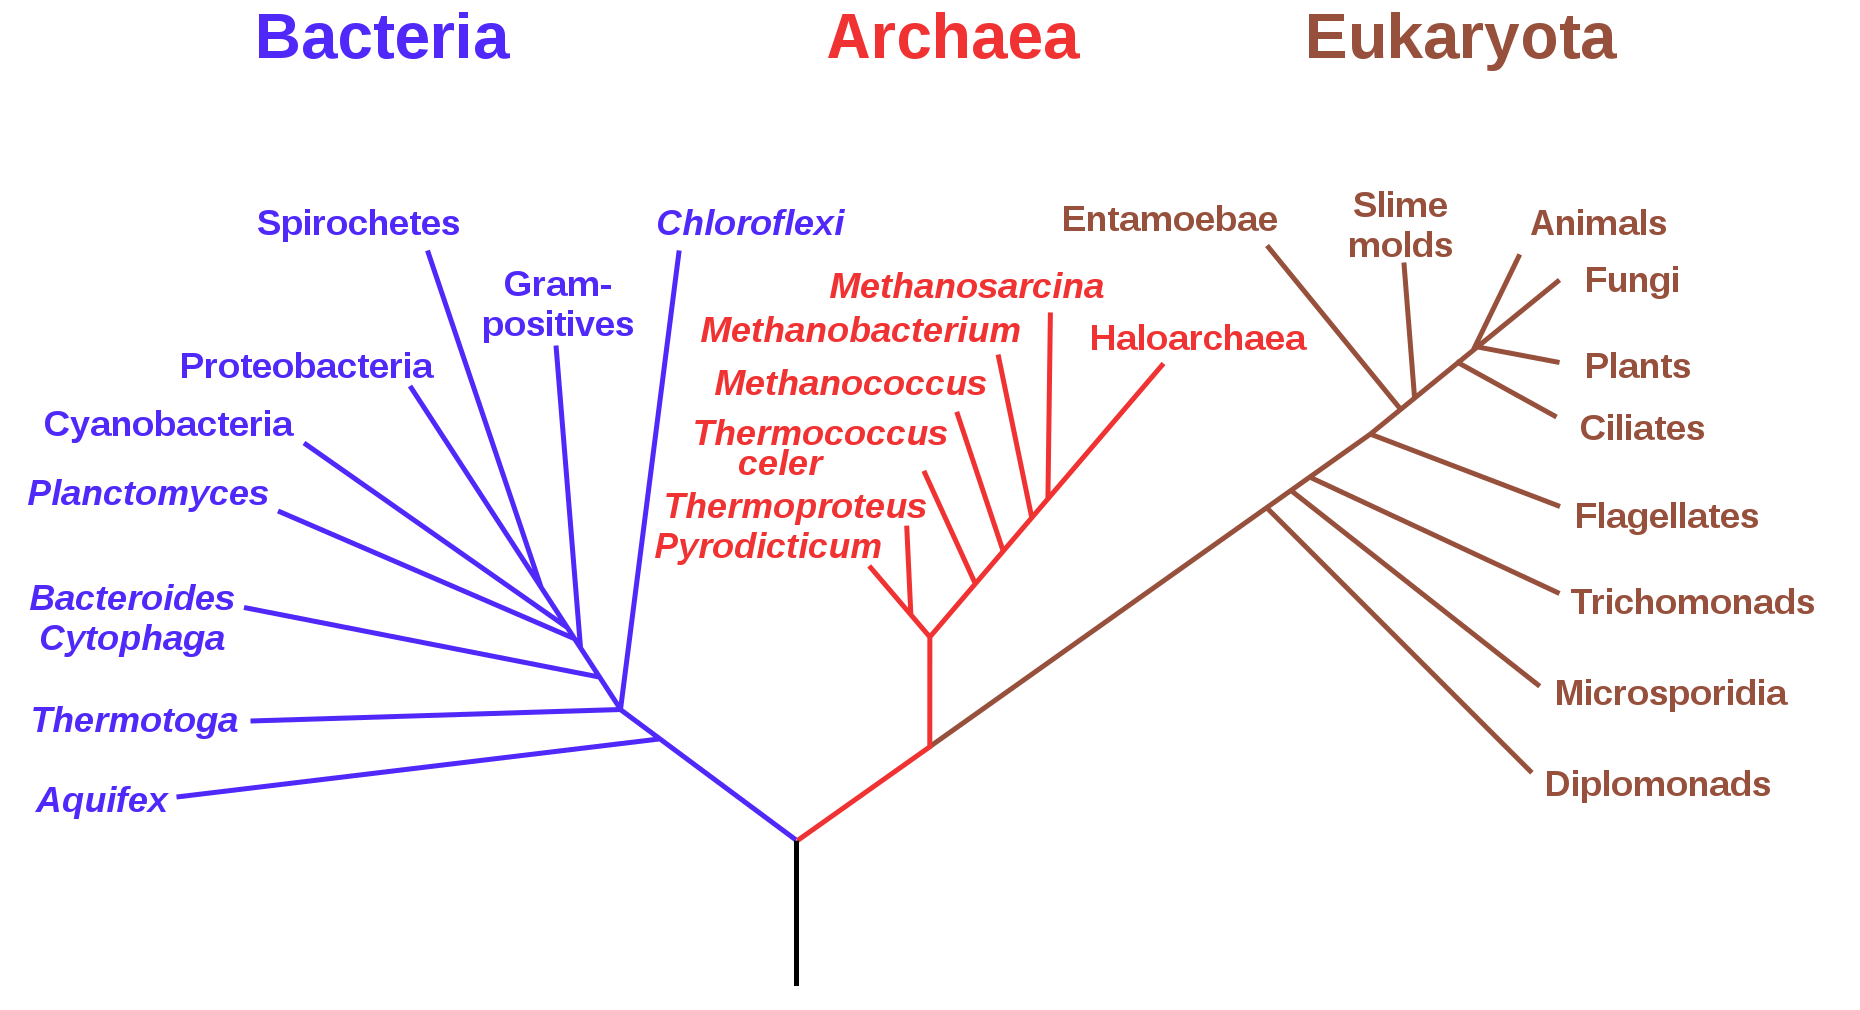
\includegraphics[width=.95\textwidth]{drvo_zivota.png}
\end{frame}

\subsection{Мрежа исхране у савани}
\begin{frame}{Мрежа исхране у савани}
\centering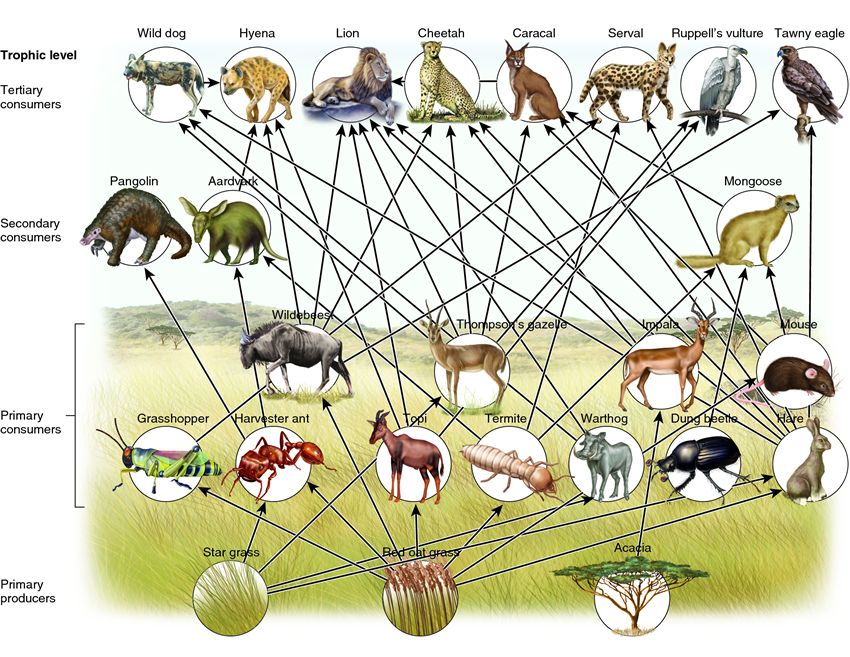
\includegraphics[width=.8\textwidth]{savana.jpeg}
\end{frame}

\subsection{Људски конектом}
\begin{frame}{Људски конектом}
\centering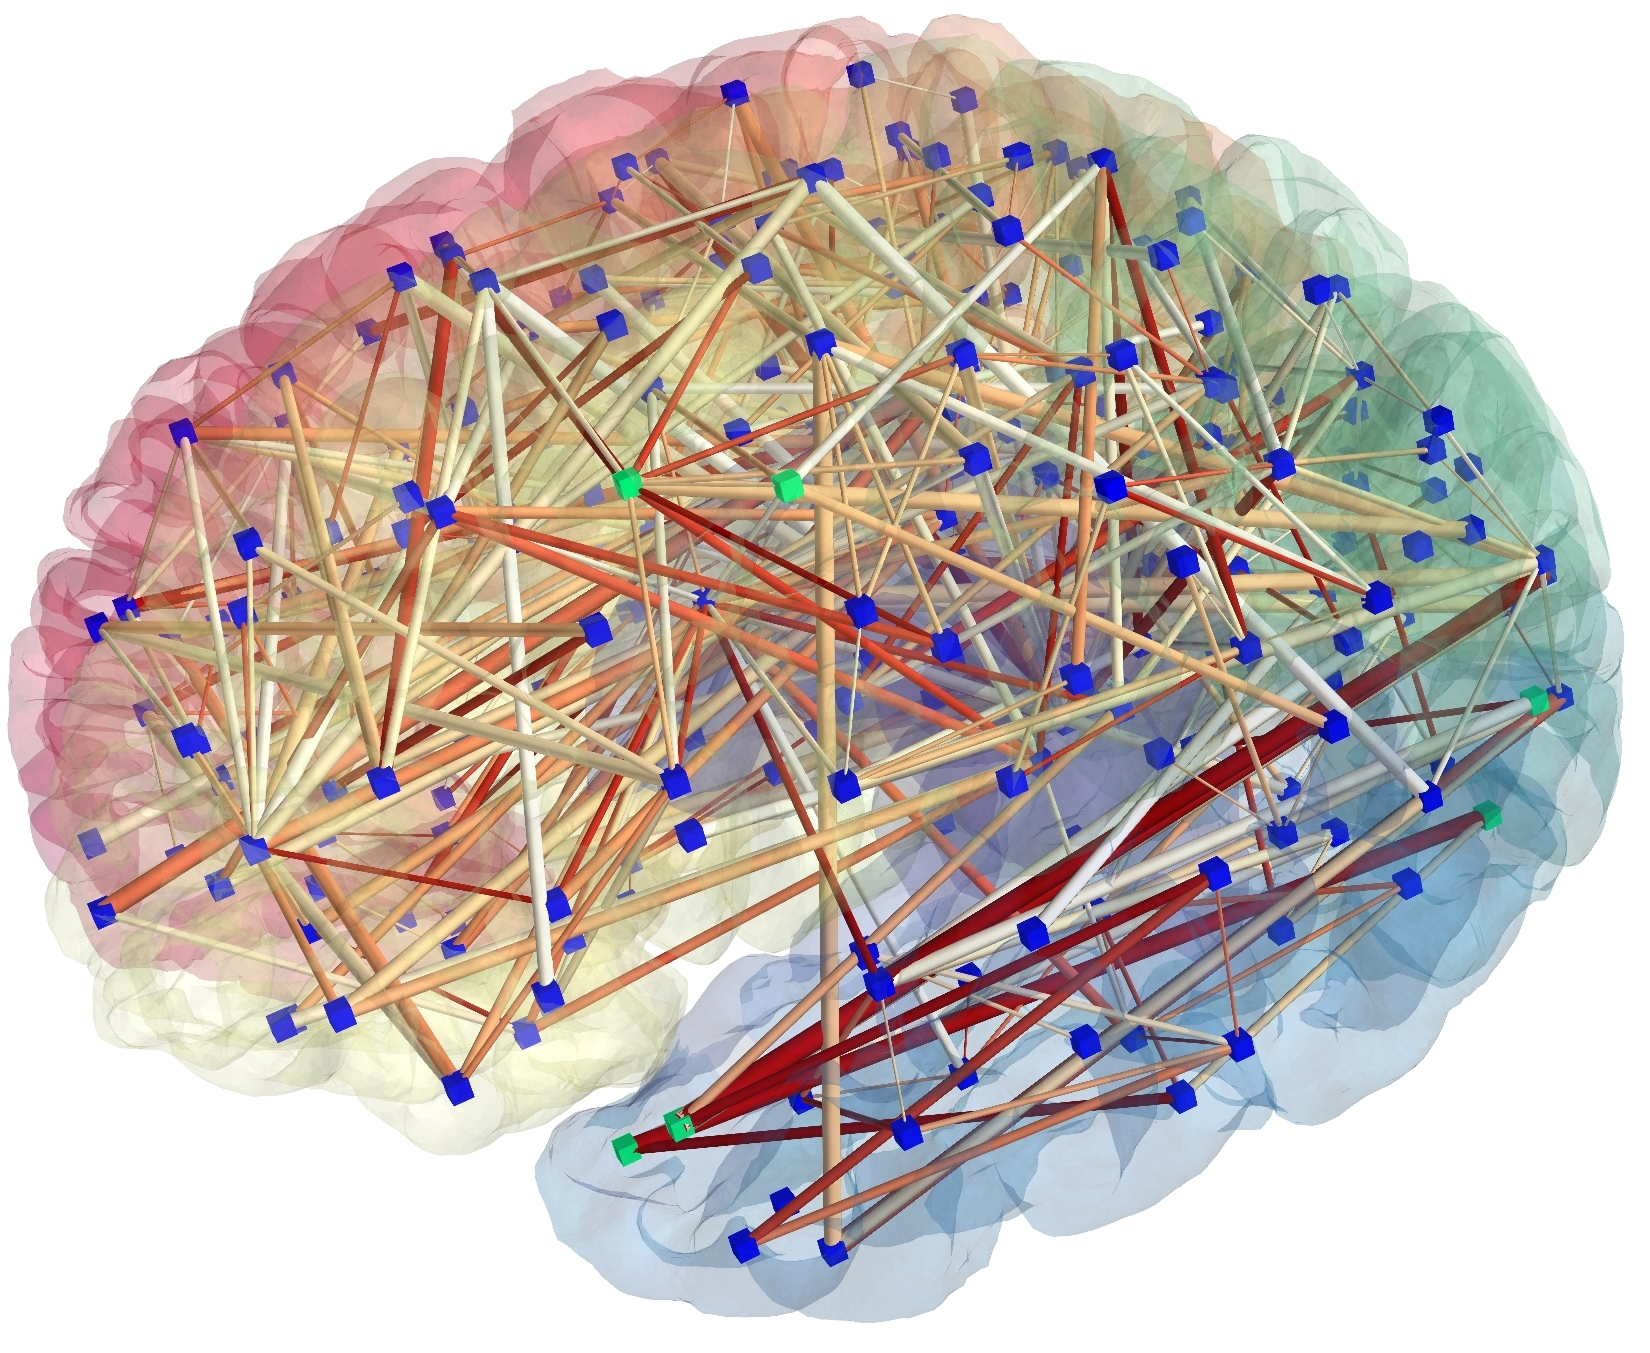
\includegraphics[width=.75\textwidth]{konektom.jpg}
\end{frame}

\section{Мреже протеинских интеракција}
\subsection{Мреже протеинских интеракција}
\begin{frame}{Мреже протеинских интеракција}
\begin{itemize}
	\item У мрежама протеинских интеракција (\textit{protein[-protein] interaction network}, $P[P]IN$), чворови су протеини, а гране неусмерене протеинске интеракције (\textit{protein-protein interaction}, $PPI$).

	\item У $PIN$ у ширем смислу, неки чворови могу бити молекули другог типа, а гране усмерене. У наставку се разматрају само уже $PPIN$ тј. $PPI$ мреже, строго са протеинима и неусмереним везама.

	\item Мрежа протеинских интеракција се једном речју назива интерактом. Слично, њени чворови се називају интеракторима, а гране интеракцијама. Област проучавања је интерактомика.
\end{itemize}
\end{frame}

\subsection{Интерактом \textit{SARS-CoV-2}}
\begin{frame}{Интерактом \textit{SARS-CoV-2}}
\centering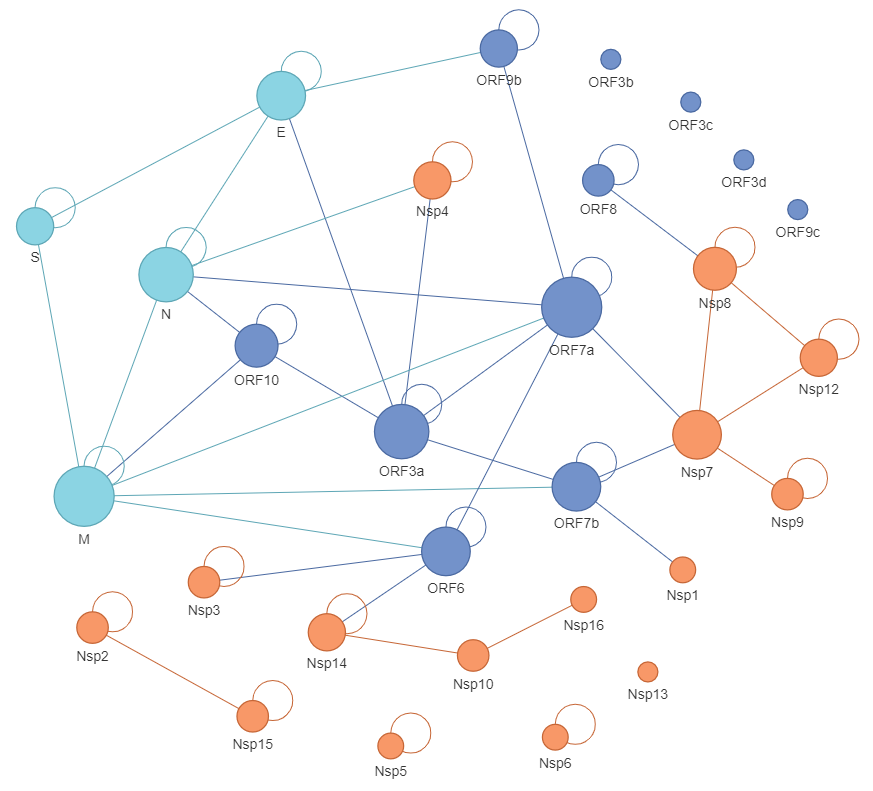
\includegraphics[width=.75\textwidth]{SARS_iRef.png}
\end{frame}

\subsection{Значај протеинских мрежа}
\begin{frame}{Значај протеинских мрежа}
\begin{itemize}
	\item Протеини обављају скоро све процесе у организму и управљају њима, при чему врло ретко делују независно. Они од виталног значаја најчешће имају више интеракција (хабови), па се лако могу идентификовати увидом у одговарајућу мрежу интеракција.

	\item Поред тога, мреже се могу поредити („поравнати”) неким од алгоритама за утврђивање сличности графова, чиме се откривају нпр. хомологне подструктуре које су очуване током еволуције.

	\item Протеини који учествују у истим ћелијским процесима или су физички спојени често су густо повезани, па се тако из мреже могу издвојити протеински комплекси. Мана: модел бинарних интеракција је превише једноставан, па су многе везе сувишне. Решење: употреба степених графова (\textit{power graph analysis}).
\end{itemize}
\end{frame}

\subsection{Ток података у интерактомици}
\begin{frame}{Ток података у интерактомици}
\centering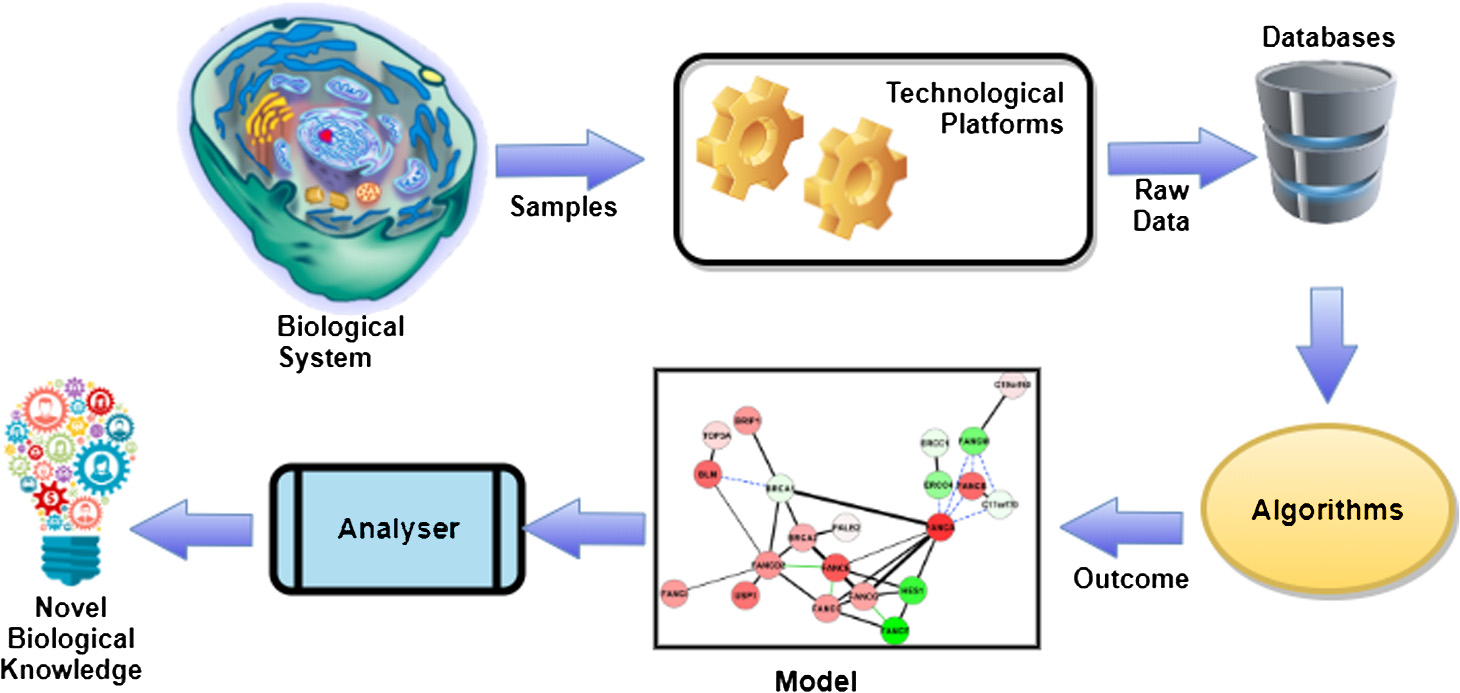
\includegraphics[width=.95\textwidth]{tok.png}
\end{frame}

\subsection{Откривање протеинских интеракција}
\begin{frame}{Откривање протеинских интеракција}
\begin{itemize}
	\item Физичке интеракције између протеина махом се откривају експериментално, у лабораторији или пак рачунарски.

	\item Рачунарским (\textit{in silico}) приступом могу се предвидети нове интеракције на основу старих, без потребе за лабораторијом. То нпр. може бити на основу сличности разматраних система.

	\item Лабораторијски приступ одликује се применом модела мамца и плена. Два најзаступљенија начина за одређивање да ли плен интерагује са мамцем јесу афинитетно прочишћавање праћено масеном спектрометријом (\textit{affinity purification -- mass spectrometry}, $AP$-$MS$) и двохибридна провера (\textit{yeast-two-hybrid}, $Y2H$).
\end{itemize}
\end{frame}

\subsection{Прочишћавање и спектрометрија}
\begin{frame}{Прочишћавање и спектрометрија}
\centering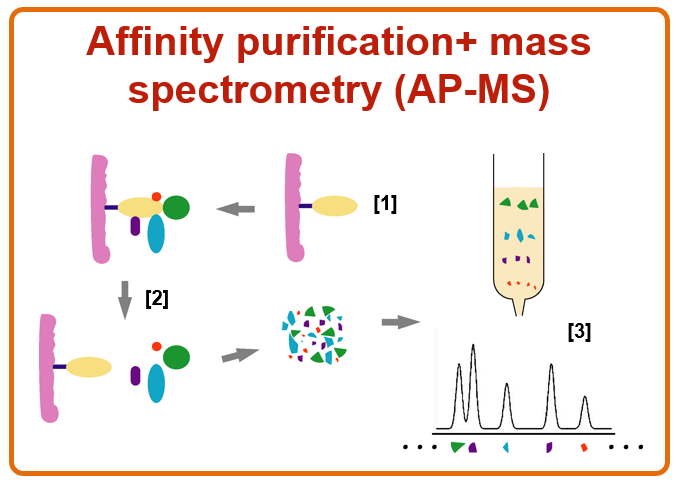
\includegraphics[width=.85\textwidth]{AP-MS.png}
\end{frame}

\subsection{Двохибридна провера}
\begin{frame}{Двохибридна провера}
\centering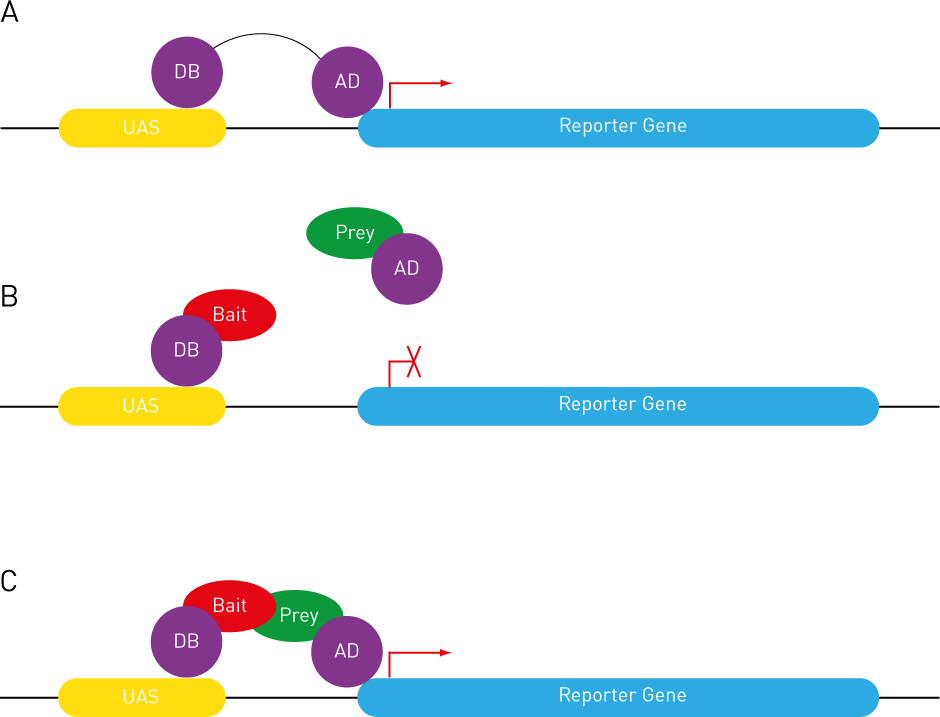
\includegraphics[width=.75\textwidth]{Y2H.png}
\end{frame}

\subsection{Базе протеинских интеракција}
\begin{frame}{Базе протеинских интеракција}
\begin{itemize}
	\item Интерактоми се могу генерисати упитом ка некој од база протеинских интеракција. Поред јавног интерфејса за дохватање списка интеракција, многе базе подржавају и графички приказ.

	\item Подаци о интеракцијама у базу се уносе ручно (експертска провера) или аутоматски, нпр. комбиновањем података из других база или анализом литературе методама истраживања текста.

	\item Неке базе (нпр. $IntAct$) интерактоме сматрају мултиграфима, при чему поновљене гране представљају везу која је потврђена у више извора. Неке базе (нпр. $STRING$) дају тежине гранама, које означавају степен сигурности у постојање интеракције.

	\item Још неке базе ($PSICQUIC$): $iRefIndex$, $MINT$, $BioGRID$...
\end{itemize}
\end{frame}

\subsection{\textit{PSICQUIC View}}
\begin{frame}{\textit{PSICQUIC View}}
\centering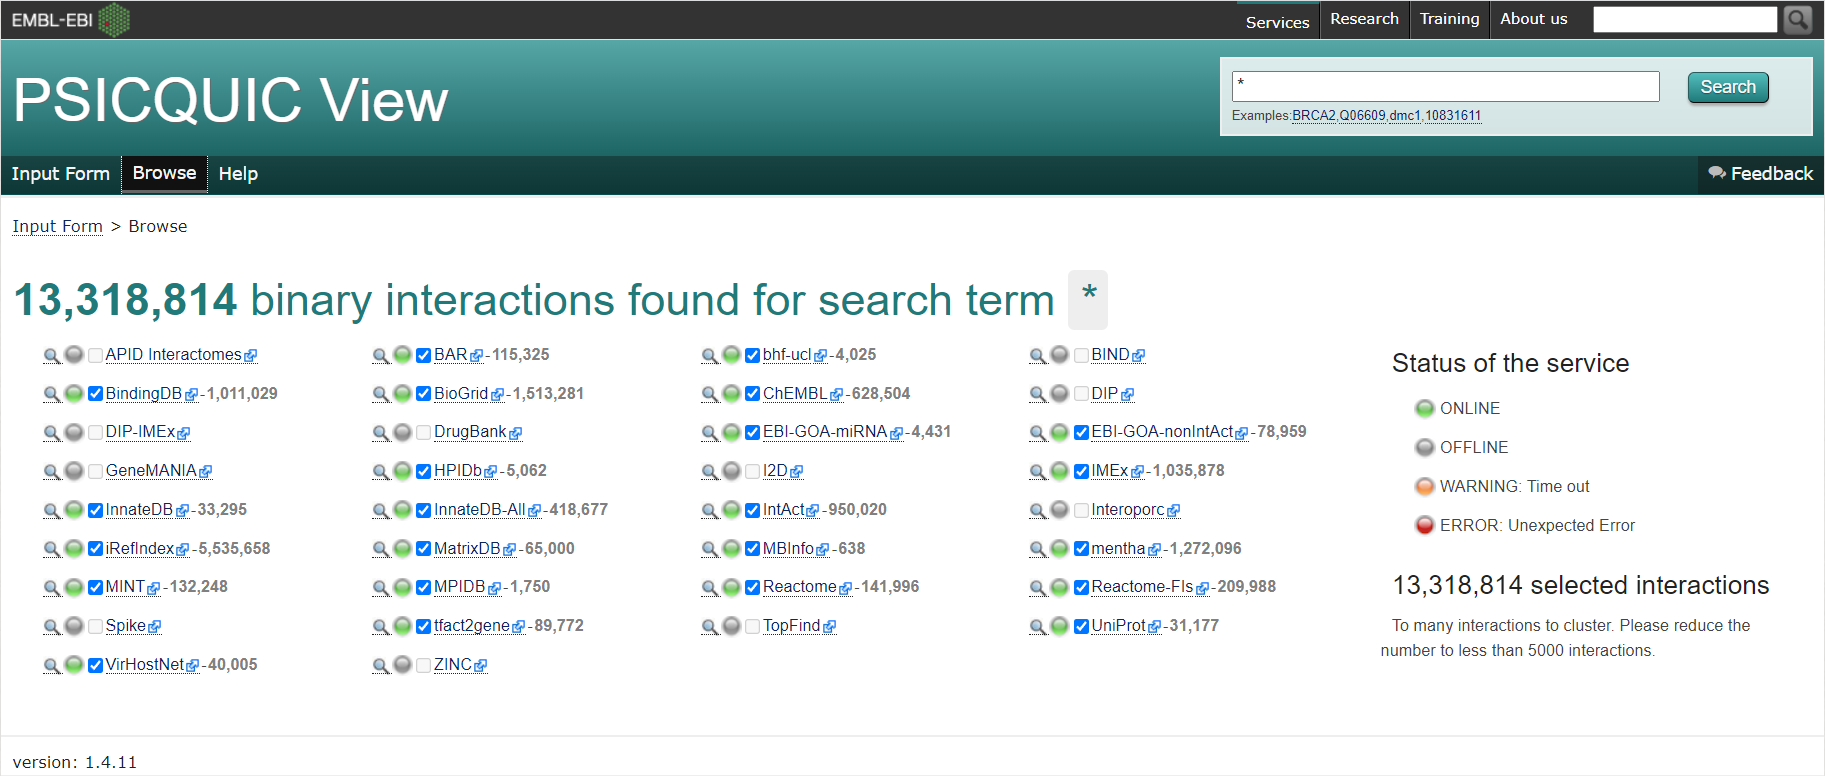
\includegraphics[width=\textwidth]{PSICQUIC.png}
\end{frame}

\subsection{$M$ протеин на $IntAct$}
\begin{frame}{$M$ протеин на $IntAct$}
\centering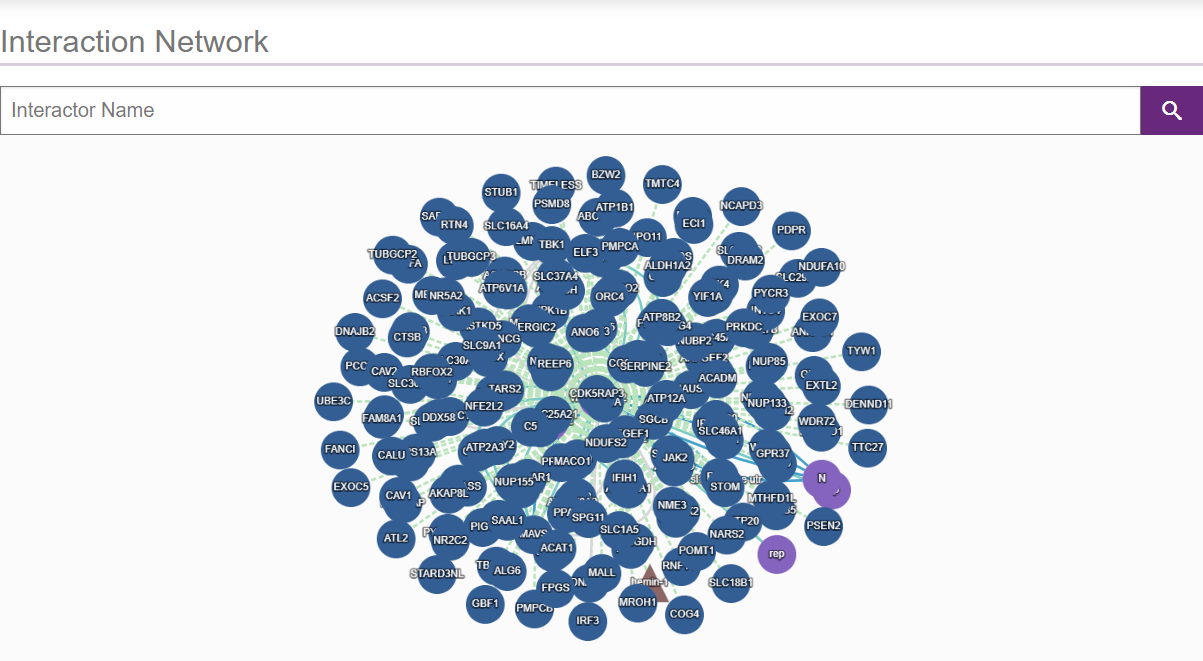
\includegraphics[width=\textwidth]{IntAct.png}
\end{frame}

\section{Неуређеност у интерактому}
\subsection{Неуређеност у интерактому}
\begin{frame}{Неуређеност у интерактому}
\begin{itemize}
	\item Неуређени протеини учествују у многобројним ћелијским процесима, па су често део великог броја интеракција. Ово значи да би потенцијално могли имати велики степен у интерактому.

	\item Проучени су интерактоми генерисани на основу одабраних протеина \textit{SARS-CoV-2}, а у њима су као особине од интереса издвојени степени повезаности и неуређености протеина.

	\item Полазни протеини: мембрански ($M$) и неструктурни ($Nsp$). Базе података: $IntAct$ и $iRefIndex$. Разматране мере неуређености: аминокиселински профил, $IUPred$, $PONDR$ и многе друге.
\end{itemize}
\end{frame}

\subsection{$Jupyter$ свеска са резултатима}
\begin{frame}{$Jupyter$ свеска са резултатима}
\centering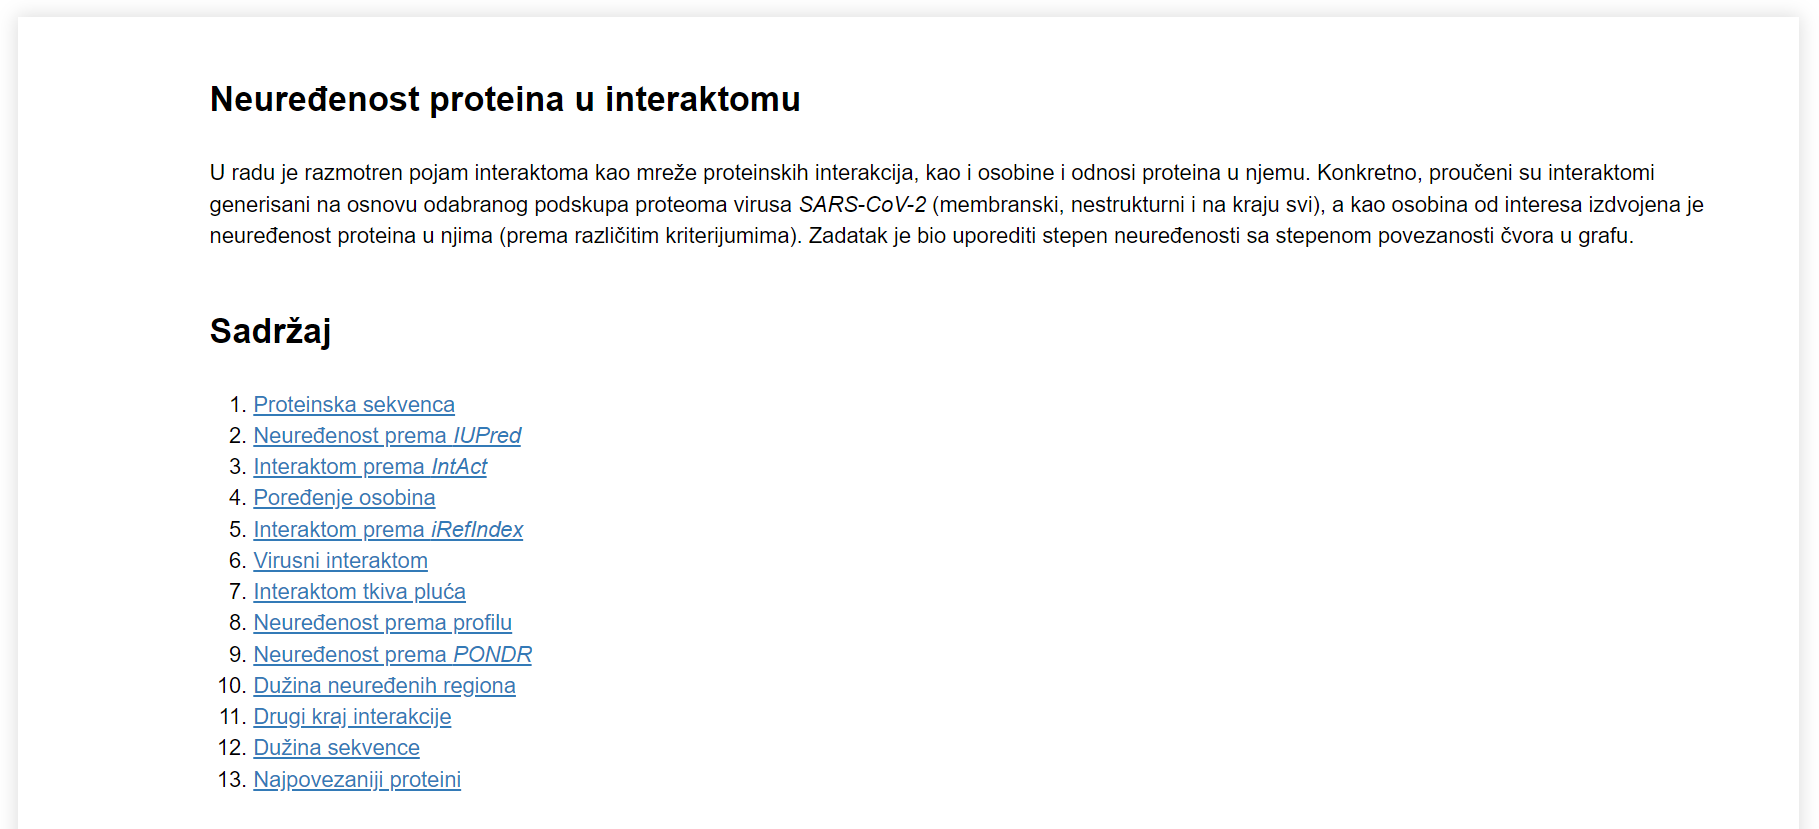
\includegraphics[width=\textwidth]{sveska.png}
\end{frame}

\addtocontents{toc}{\protect\setcounter{tocdepth}{-1}}

\section{Закључак}
\subsection{Закључак}
\begin{frame}{Закључак}
\begin{itemize}
	\item Будући интерагујући блокови, биолошки системи се природно моделују графовима (мрежама). Резултујуће мреже су разноврсне по природи, али имају специфичне тополошке карактеристике.

	\item Мреже протеинских интеракција (интерактоми) моделују односе протеина (интерактора). Њиховом биоинформатичком анализом могуће је доћи до нових знања о разматраним протеинима.

	\item На примеру анализе неуређености протеина у интерактомима генерисаним на основу одабраних протеина вируса \textit{SARS-CoV-2}, приказан је целокупан ток података у интерактомици.
\end{itemize}
\end{frame}

\subsection{Литература}
\begin{frame}{Литература}
\nocite{*}
\bibliographystyle{amsalpha}
\bibliography{Interaktomika}
\end{frame}

\end{document}